% METODOLOGIA------------------------------------------------------------------

\chapter{DESENVOLVIMENTO}
\label{chap:metodologia}

\textcolor{red}{TODO: intro}

Este capítulo aborda o desenvolvimento do projeto.

\section{CONCEPÇÃO DO PROJETO}
\label{sec:concepcao}

Com base no projeto arquitetônico e a partir do levantamento das tecnologias disponíveis e viáveis (sobretudo pelo custo e pela difusão no mercado), foram definidos os componentes e técnicas a serem utilizadas no projeto eletrônico, cujo diagrama geral é apresentado na \autoref{fig:diagramageral}.

\begin{figure}[H]
    \centering
    \caption{Diagrama geral do projeto eletrônico}
    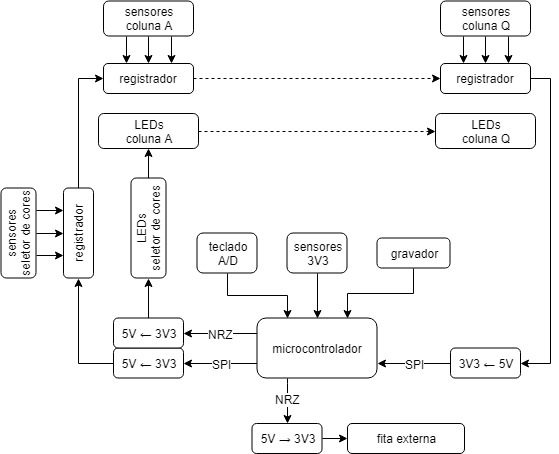
\includegraphics[width=0.8\textwidth]{./dados/figuras/diagrama}
    \fonte{(O AUTOR, 2018)}
    \label{fig:diagramageral}
\end{figure}

A partir do projeto arquitetônico (\autoref{fig:mesa-sup}), que é segmentado em duas partes: Matriz (interação) e Controle (seletor de cores), o projeto eletrônico também foi organizado em 3 subdivisões: Matriz, Interface e Controlador, apresentadas na \autoref{fig:subsecoes}. Dessa forma, pôde-se dar andamento ao projeto por meio de etapas, onde cada fase pode ser considerada um projeto íntegro por si só.

\begin{figure}[H]
    \centering
    \caption{As 3 subseções principais do projeto eletrônico}
    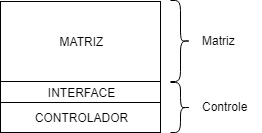
\includegraphics[width=0.45\textwidth]{./dados/figuras/secoes}
    \fonte{(O AUTOR, 2018)}
    \label{fig:subsecoes}
\end{figure}

As subdivisões têm funções bem definidas, apresentadas logo abaixo, e serão discutidas neste mesmo capítulo nos tópicos a seguir.

\begin{itemize}
    \item \textbf{Matriz:} é o setor que pode ser ``pintado com luz'', que contém os LEDs e os sensores de interação. É inteiramente comandada pelo Controlador, através da Interface;
    \item \textbf{Interface:} interliga as subseções Matriz e Controlador. Captura e propaga o sinal dos sensores, através dos registradores de deslocamento, e forma a ligação sequencial do barramento dos LEDs;
    \item \textbf{Controlador:} processa todos os LEDs e sensores da mesa. Contém os LEDs e os sensores do seletor de cores, a parte de processamento, os conversores de nível lógico e os periféricos de gravação e depuração.
\end{itemize}

\textcolor{red}{TODO: especificações, tensão}

\textcolor{red}{TODO: software}

\section{PROJETO DA MATRIZ}
\label{sec:matriz}

O projeto da Matriz foi concebido durante o Programa de Iniciação Científica do qual o autor participou. Nele, o desafio foi o de contemplar todas as 118 bolinhas de \emph{ping-pong} desta seção (e seus respectivos pares sensor-LED), visando robustez e o menor custo.

Para tal, foi definido que a matriz seria arranjada em 17 colunas verticais, conforme apresentado na \autoref{fig:placas-matriz-colunas}. Consequentemente, devido à disposição dos objetos (determinada pelo projeto arquitetônico), essas colunas poderiam conter 5, 6, 7 ou 8 bolinhas e, para abrangê-las da maneira mais proveitosa, as colunas foram combinadas por módulos (placas) de 2 ou 3 bolinhas.

Em geral, as empresas fabricantes de placas de circuito impresso consideram cada modelo de placa como um projeto, devido ao corte do painel, procedimento para os testes elétricos e etc. Assim, utilizando-se de apenas 2 modelos de placa, foi possível reduzir o custo do projeto sem dispensar a robustez que as PCIs proporcionam.

\begin{figure}[H]
    \centering
    \caption{Disposição das placas da Matriz}
    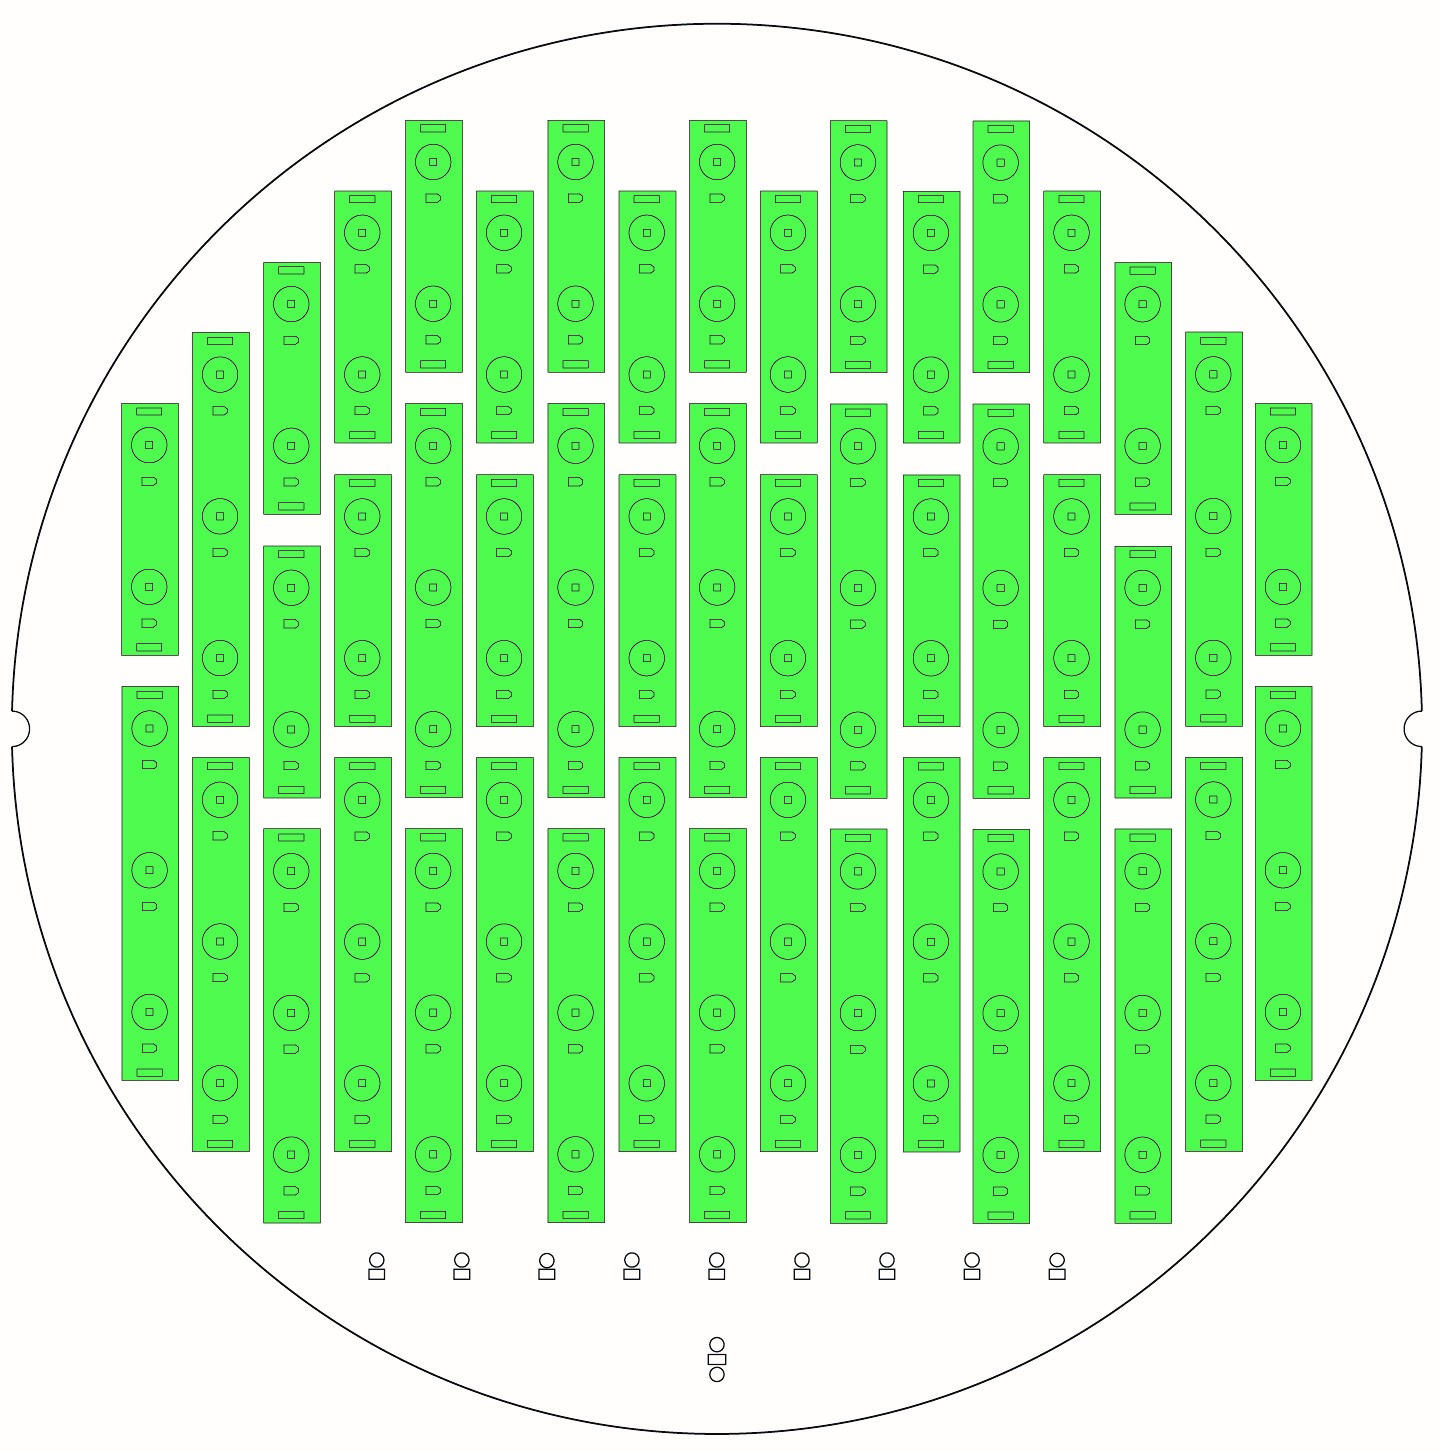
\includegraphics[width=0.7\textwidth]{./dados/figuras/placas-matriz-colunas}
    \fonte{(O AUTOR, 2017)}
    \label{fig:placas-matriz-colunas}
\end{figure}

Uma vez definido que a matriz seria composta por placas com 2 ou 3 bolinhas, iniciaram-se os testes de conceito com o protótipo apresentado na \autoref{fig:matriz-prototipo}. Nesses ensaios, foram testados os conceitos de endereçamento do LED WS2812, a leitura do nível lógico dos sensores através dos registradores de deslocamento e também o modo de conexão entre as placas.

\begin{figure}[H]
    \centering
    \caption{Protótipo das placas da matriz}
    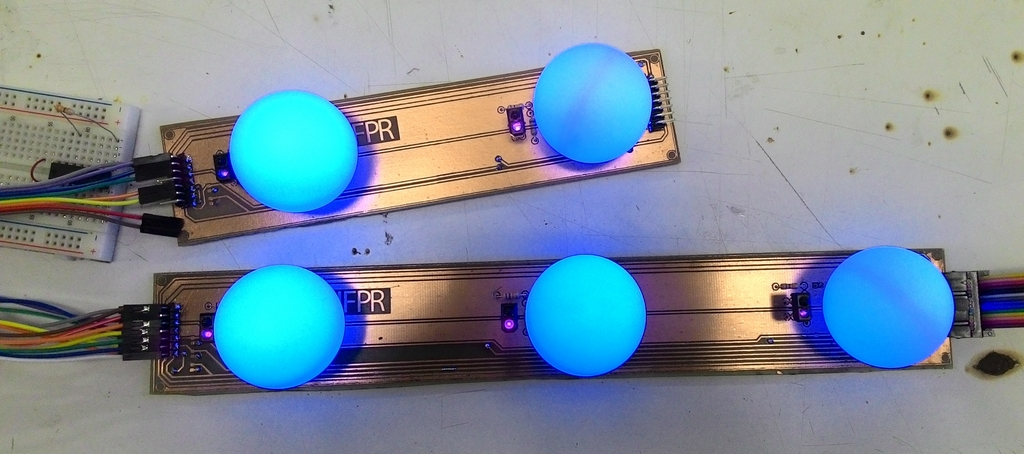
\includegraphics[width=0.8\textwidth]{./dados/figuras/mesa-protoboard}
    \fonte{(O AUTOR, 2017)}
    \label{fig:matriz-prototipo}
\end{figure}

Todos os conceitos propostos foram validados e as 47 placas que compõem a matriz foram confeccionadas em produção industrial. A \autoref{fig:placa2} e a \autoref{fig:placa3} apresentam as faces superior e inferior dos módulos.

\begin{figure}[H]
    \centering
    \caption{Faces da PCI do módulo de 2 bolinhas}
    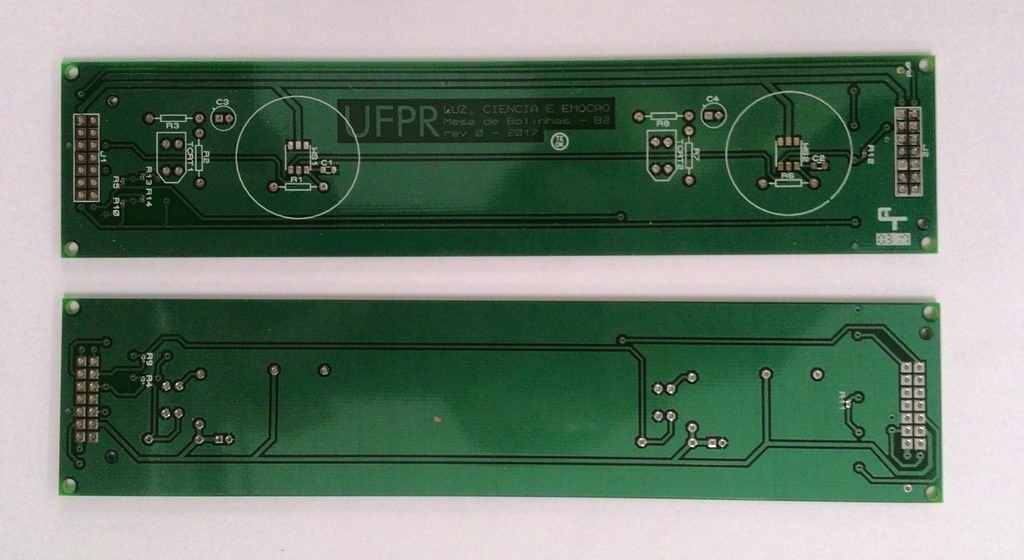
\includegraphics[width=0.8\textwidth]{./dados/figuras/bloco-2}
    \fonte{(O AUTOR, 2017)}
    \label{fig:placa2}
\end{figure}

\begin{figure}[H]
    \centering
    \caption{Faces da PCI do módulo de 3 bolinhas}
    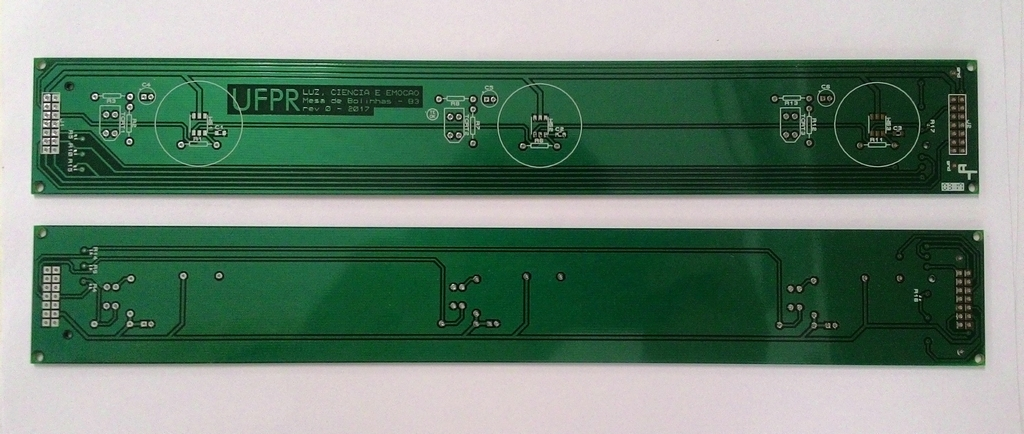
\includegraphics[width=0.99\textwidth]{./dados/figuras/bloco-3}
    \fonte{(O AUTOR, 2017)}
    \label{fig:placa3}
\end{figure}

\textcolor{red}{TODO: consumo da mesa}

\section{PROJETO DA INTERFACE}
\label{sec:interface}

Como já brevemente introduzido pela \autoref{sec:concepcao} (Concepção do Projeto), a Interface tem a função de interligar as seções Matriz e Controlador. Contudo, deve-se atentar a algumas questões:

\begin{enumerate}[label=\Roman*.]
    \item Os LEDs devem formar um barramento sequencial da esquerda para a direita; de baixo para cima;
    \item A referência de cada sensor deve ser embarcada no barramento na mesma ordem que os LEDs;
    \item Por integrar dois barrementos de frequências razoáveis (NRZ @800kHz e SPI @4MHz, LEDs e sensores respectivamente), deve-se evitar construir trilhas com quinas abruptas, em função da reflexão do sinal;
    \item As trilhas de potência devem ser adequedas para aguentarem a corrente no caso mais extremo.
\end{enumerate}



\textcolor{red}{TODO: NET TIE}

\textcolor{red}{TODO: diagrama com 9 registradore, 8 registradores, placa 1, placa 2}

\textcolor{red}{TODO: um com 9, outro com 8, configuração através do resistor direcionador}

\subsection{PROJETO DA PCI DA INTERFACE}
\label{subsec:pciinterface}

\textcolor{red}{TODO: 2D placa}

\textcolor{red}{TODO: roteamento trilhas curvadas, dupla face FR4}

\textcolor{red}{TODO: net tie}

\textcolor{red}{TODO: 3D da placa}

\section{PROJETO DO CONTROLADOR}
\label{sec:controlador}

\textcolor{red}{TODO: diagrama simplificado}

\subsection{ALIMENTAÇÃO}
\label{subsec:alimentacao}

\textcolor{red}{TODO: separação das alimentações}

\textcolor{red}{TODO: fonte (diodo proteção)}

\textcolor{red}{TODO: net tie}

\subsection{SELETOR DE CORES}
\label{subse:seletor}

\textcolor{red}{TODO: shift register com os sensores}

\textcolor{red}{TODO: conversor de nível saída, baker clamp}

\textcolor{red}{TODO: sensores 3v3}

\subsection{TECLADO ADC}
\label{subsec:tecladoadc}

\subsection{GRAVADOR}
\label{subsec:gravador}

\textcolor{red}{TODO: comunicação serial}

\textcolor{red}{TODO: botões}

\textcolor{red}{TODO: tabela função XOR? que substitui os botões}

\textcolor{red}{TODO: ftdi}

\subsection{PROJETO DA PCI DO CONTROLADOR}
\label{subsec:pcicontrol}

\textcolor{red}{TODO: 2D PCI controlador}

\textcolor{red}{TODO: NET TIE}

\textcolor{red}{TODO: 3D PCI controlador}

\section{PROJETO DO \emph{FIRMWARE}}
\label{sec:firmware}

\subsection{\emph{DEBOUNCE}}
\label{subsec:debounce}

\subsection{MÁQUINA DE ESTADOS FINITA}
\label{subsec:fsm}

\textcolor{red}{TODO: citar a referencia gang  of 4}

